% Author: Dominik Harmim <xharmi00@stud.fit.vutbr.cz>


\documentclass[11.5pt]{article}
\usepackage{hyperref}
\usepackage{url}
\usepackage{sidecap}
\usepackage{float}
\usepackage[backend=biber]{biblatex}
\addbibresource{zdroje.bib}

\usepackage[margin=3cm]{geometry}
\usepackage[czech]{babel}
\usepackage[utf8]{inputenc}
\usepackage{times}
\usepackage{graphicx}
\usepackage[unicode]{hyperref}
\hypersetup{
	colorlinks = true,
	hypertexnames = false,
	citecolor = red
}


\begin{document}
	%%%%%%%%%%%%%%%%%%%%%%%%%%%%%%%% Titulní stránka %%%%%%%%%%%%%%%%%%%%%%%%%%%
	\begin{titlepage}
		\begin{center}
			
\includegraphics[width=0.77\linewidth]{pic/FIT_logo.pdf} \\

			\vspace{\stretch{0.382}}

			\Huge{Dokumentace} \\
			\LARGE{\textbf{
				ESP32: Měření srdečního tepu [analogový senzor]
			}} \\
			\Large{Mikroprocesorové a vestavěné systémy}

			\vspace{\stretch{0.618}}
		\end{center}

		{\Large            
            Adam Kala (xkalaa00)
            \hfill
            \today
		}
	\end{titlepage}



	%%%%%%%%%%%%%%%%%%%%%%%%%%%%%%%% Obsah %%%%%%%%%%%%%%%%%%%%%%%%%%%%%%%%%%%%%
         \tableofcontents
        \addtocontents{toc}{\protect\thispagestyle{empty}}
	\clearpage



	%%%%%%%%%%%%%%%%%%%%%%%%%%%%%%%% Úvod %%%%%%%%%%%%%%%%%%%%%%%%%%%%%%%%%%%%%%
	
	\section{Úvod}
        \pagenumbering{arabic}
	\setcounter{page}{1}
        Cilém projektu bylo s využitím vývojového kitu Espressif ESP32 \cite{esp32}, snímačem srdečního tepu PulseSensor \cite{snimac}, grafického OLED displeje \cite{displej}
        a vývojového prostředi Arduino zrealizovat systém pro měření srdečního tepu. 

        Použitý senzor srdečního tepu generuje analogový výstup, který je konvertován na digitální podobu pomocí analogově-digitálního převodníku uvnitř mikrokontroléru ESP32. 

        \section{Vývojové prostředí}
        Projekt byl vyvíjen ve Visual Studio Code ve spojení s PlatformIO, jenž zajišťovalo správu knihoven, nahrávání kódu na hardware a integraci s mikrokontrolérem ESP32.

        \section{Zapojení hardwaru}\label{zapojeni}
        
        \subsection{OLED displej}
        Displej byl zapojen do pinů SCL a SDA. Nápajení probíha přes 5V (+) a GND (-), viz. obrázek \ref{fig:esp32}.
        \subsection{Snímač srdečního tepu PulseSensor}
        Snímáč byl také napájen přes 5V (+) a GND (-), jeho signál byl zapojen do pinu 36 (ADC0), viz. obrázek \ref{fig:esp32}.
        \begin{figure}[H]
          \centering
          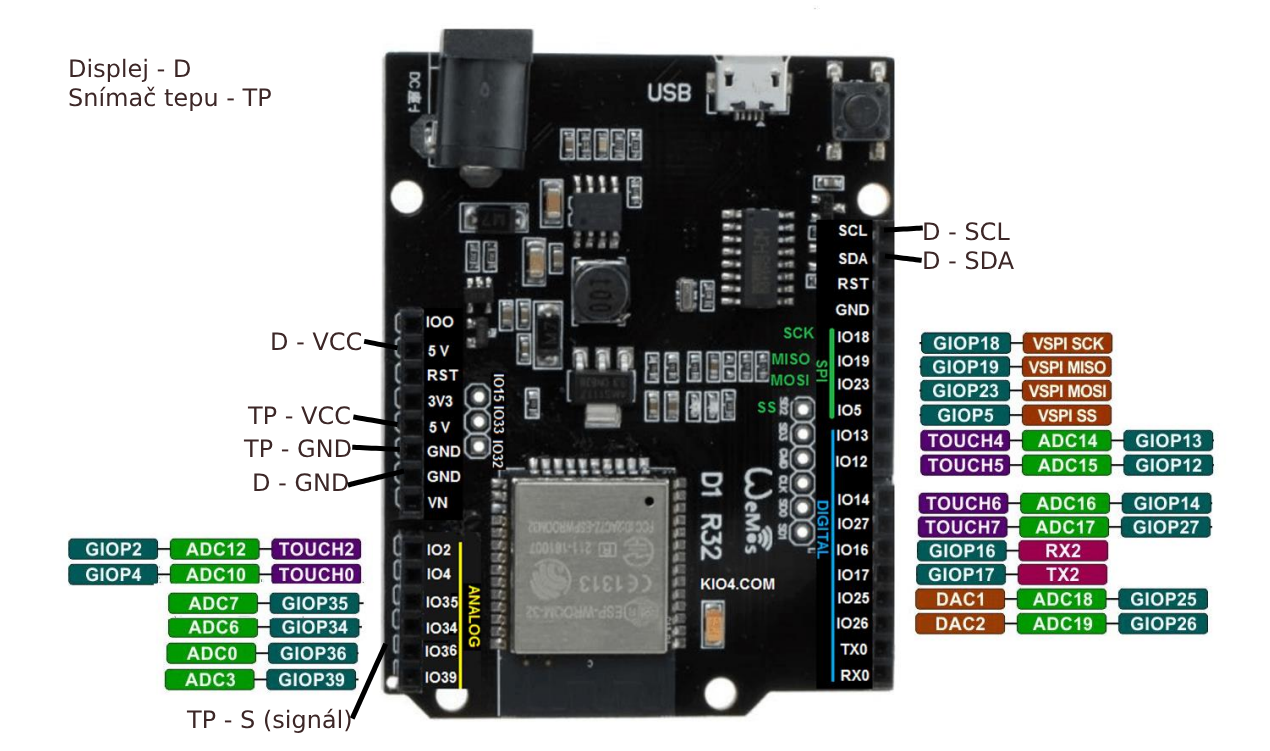
\includegraphics[width=\linewidth]{pic/deska.png}
          \caption{Návrh zapojení desky ESP32}
        \end{figure}

        \begin{figure}[H]
          \centering
          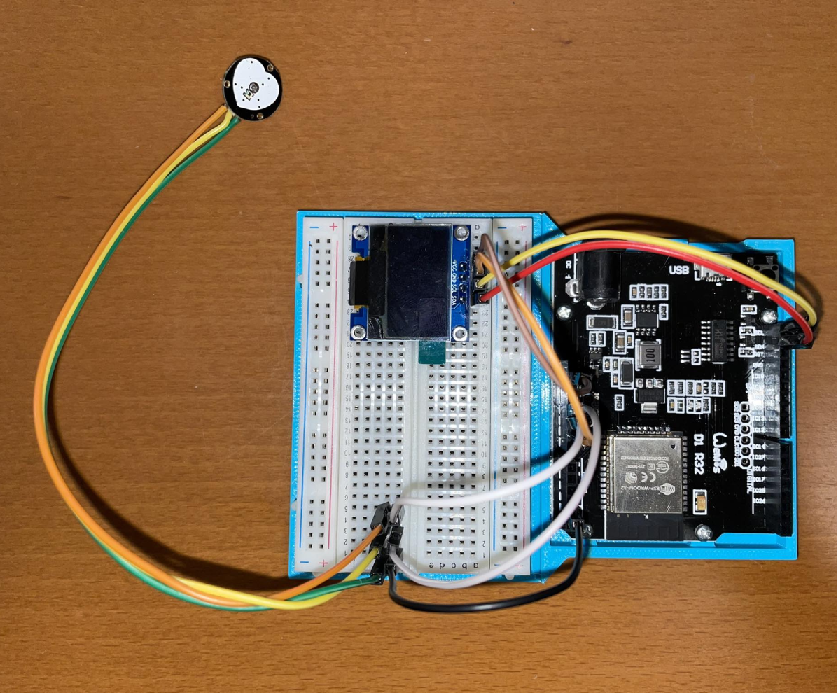
\includegraphics[width=\linewidth]{pic/zapojeni.png}
          \caption{Realizace zapojení desky ESP32}
          \label{fig:esp32}
        \end{figure}

    \section{Potíže}
        Zapojení desky a následná konfigurace prostředí bylo bez zaváhání. Problém přišel u samotného snímače tepu, který rád ukazoval hodnoty až nesmyslné. Vždy také chvíli trvalo, než si 
        prst \uv{odchytl} a začal ukazovat požadované hodnoty.

    \section{Řešení}
        Program využívá knihoven \texttt{Arduino.h}, \texttt{Wire.h} a \texttt{Adafruit\_SSD1306.h} pro jednoduché ovládání displeje, jenž je nainicializován na začátku kódu. Dále je definovaná proměnná \texttt{PULSE\_SENSOR\_PIN}, která je nastavena na hodnotu 36, podle zapojení zmíněného v kapitole \ref{zapojeni}, a \texttt{NUMBER\_OF\_VALS} na 500, která bude později použita pro samotné odchytávání tepu.

        Program nejprve vstoupí do funkce \texttt{setup()}, ve které se nastaví sériová komunikace na 9600 baudů (počet změn signálu za sekundu). Dále je poprvé nastaven displej na port 0x3C a 2 sekundové zpoždění, aby nastavení proběhlo v pořádku.

        Všechno získávání hodnot probíhá v nekonečném cyklu, který po dobu 10 sekund (500/20ms zpoždění) získává hodnoty ze senzoru (přes funcki \texttt{analogRead()}), kterou uložíme do pole \texttt{values}. Dále se v tomto cyklu také odečítá celkový čas z měření, který se postupně zobrazuje na displeji v hodnotách 9 (začátek měření) až 0 (konec měření).

        Pro dosaženích lepších výsledků jsem se rozhodl naimplementovat jednoduchý mediánový filtr, který prochází již zmíněné hodnoty, porovná je, seřadí vzestupně a nakonec vrátí hodnotu uprostřed pole. Tato metoda mi přinesla lepší výsledky než počítaní průměru, jelikož tam nejsou zahrnovány extrémní výkyvy senzoru.

        Po aplikování mediánového filtru program porovnává tuto hodnotu, zvýšenou o 40 (toto číslo fungovalo nejspolehlivěji), s hodnotami naměřenými z \texttt{analogRead()}. Při každém nálezu vyšší hodnoty inkrementuji  proměnnou \texttt{anomally} o 1.

        V závěru cyklu se hodnota \texttt{anomally} vynásobí 6, abychom dosáhli hodnoty za minutu. Dále jsem nastavil spodní hranici tepu na 40 a horní na 200, aby byl program ještě o trochu spolehlivější. 
        
        \section{Funkcionalita a testování}
        Displej na začátku zobrazuje 0, poté naposledy naměřenou hodnotu společně s odpočtem právě probíhajícího měření.
        
        Testování probíhalo při celé implementaci programu. Tep byl porovnáván s hodnotami, které by měly odpovídat mému fyzickému stavu. Avšak hodnoty se mohou lišit vzhledem k momentálnímu stavu jedince, jenž může být ovlivněn například stresem, únavou, množstvím užitého kofeinu, atd.
        \begin{itemize}
            \item{Klidový stav: 50 - 100}
            \item{Fyzická námaha: 100 - 150}
        \end{itemize}
        U konečných testů byl zkoušen klidový tep (tep se snižoval s délkou klidového stavu) a tep po fyzické námaze. Tyto testy jsem zdokumentoval pomocí videa a nahrál na Google Drive.
        \subsubsection*{Odkazy na testování:}
        \href{https://drive.google.com/file/d/1SJeyl9q0O1pvIM8aHSfGlxWqP7FoRAWI/view?usp=drive_link}{Snižující se klidový tep}\\
        \href{https://drive.google.com/file/d/1o8epXSymkZcHvcDapgJTr4hES4HnGgzo/view?usp=drive_link}{Tep po fyzické námaze}\\
        \\
        Problém s odkazy? Použijte \nameref{testproblem}.
    \section{Závěr}
        Projekt byl svou náplní jeden z těch zábavnějších. Jeho řešení je za správné funkčnosti senzoru odpovídající. V některých případech ale trvá, než si senzor sedne a začne snímat adekvátní hodnoty. 
	%%%%%%%%%%%%%%%%%%%%%%%%%%%%%%%% Citace %%%%%%%%%%%%%%%%%%%%%%%%%%%%%%%%%%%%
    \clearpage
    \section{Zdroje}
    Při realizaci projektu bylo čerpáno z těchto zdrojů: \cite{displej} \cite{snimac} \cite{esp32} \cite{pulsesensortutorial} \cite{sensorusingarduino}\\
    \\
    \label{testproblem}Při problémech s hypertextovým odkazem u testování, použijte:\\
    \url{https://drive.google.com/file/d/1o8epXSymkZcHvcDapgJTr4hES4HnGgzo/view?usp=drive_link}\\
    \url{https://drive.google.com/file/d/1SJeyl9q0O1pvIM8aHSfGlxWqP7FoRAWI/view?usp=drive_link}
    
    \printbibliography
	
\end{document}

